% 60-15(인쇄 60쪽) — 평행한 두 직선 l, m 과 그 위의 점 5개·2개. 스캔 그림을 TikZ 로 다시 그림.
% 점에는 원문처럼 이름을 붙이지 않고, 라벨은 직선 이름 l·m 둘뿐이다(삼각형 개수 등 답의 근거는 적지 않는다).
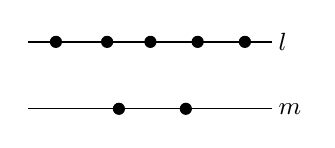
\begin{tikzpicture}[line width=0.5pt]
  \draw (0,0.85) -- (3.1,0.85);
  \foreach \x in {0.35,1.0,1.55,2.15,2.75} \fill (\x,0.85) circle (2.2pt);
  \node[anchor=west, inner sep=2pt, font=\small] at (3.1,0.85) {$l$};
  \draw (0,0) -- (3.1,0);
  \foreach \x in {1.15,2.0} \fill (\x,0) circle (2.2pt);
  \node[anchor=west, inner sep=2pt, font=\small] at (3.1,0) {$m$};
\end{tikzpicture}
